\subsection{Properties of Functions: Increasing or Decreasing}
\begin{definition}[Increasing]
  $$for\: x_1 < x_2$$
  $$f(x_1) < f(x_2)$$
  From $left \to right$ in the $x$-axis, the graph climbs upward.
\end{definition}

\begin{definition}[Decreasing]
  $$for\: x_1 < x_2$$
  $$f(x_1) > f(x_2)$$
  From $left \to right$ in the $x$-axis, the graph falls downward.
\end{definition}

\textbf{Note: }All of this is given by an open intervals of the $x$-axes.

\begin{example}[Decreasing and Increasing Function] 
  \hfill
  \begin{center}
    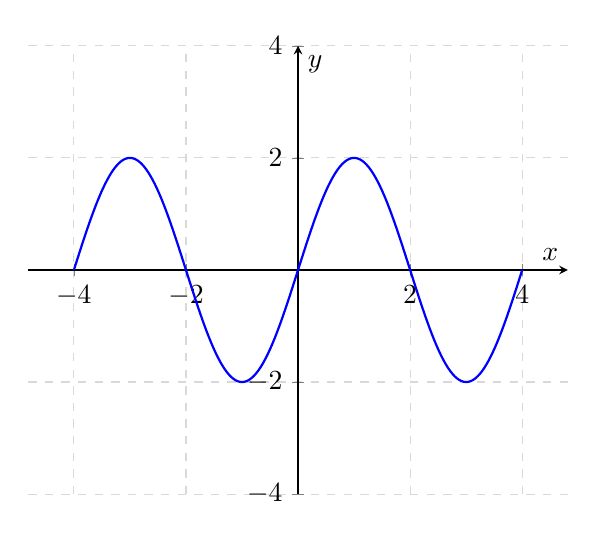
\begin{tikzpicture}
      \begin{axis}[
	  axis lines = center,
	  xlabel = $x$,
	  ylabel = $y$,
	  xmin = -4, xmax = 4,
	  ymin = -4, ymax = 4,
	  grid = both,
	  grid style = {dashed, gray!30},
	  axis equal
	]
	\addplot [domain=-4:4, samples=200, thick, blue] {2*sin(deg(pi/2*x))};
      \end{axis}
    \end{tikzpicture}
  \end{center}
  $$Increasing\: [-1, 1] \cup [3, 4]$$
  $$Decreasing\: [-3, -1] \cup [1, 3]$$

  Another example is:
  $$f(x) = -x^3 - 3*x$$
  \hfill
  \begin{center}
    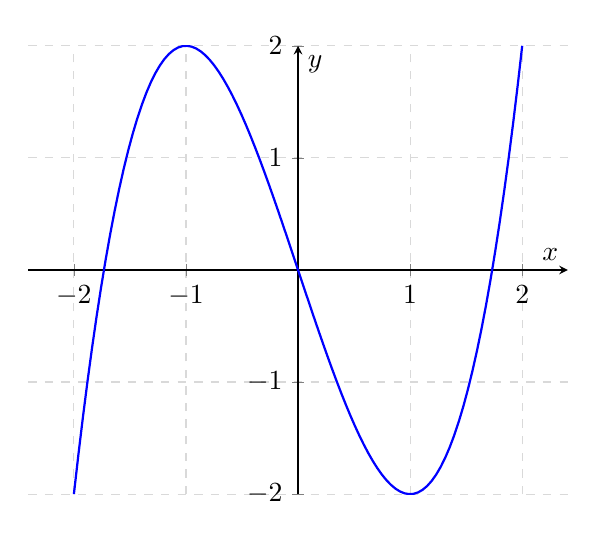
\begin{tikzpicture}
      \begin{axis}[
	  axis lines = center,
	  xlabel = $x$,
	  ylabel = $y$,
	  xmin = -2, xmax = 2,
	  ymin = -2, ymax = 2,
	  grid = both,
	  grid style = {dashed, gray!30},
	  axis equal
	]
	\addplot [domain=-2:2, samples=100, thick, blue] {x^3 - 3*x};
      \end{axis}
    \end{tikzpicture}
  \end{center}
  $$Increasing\: [-1, 1]$$
  $$Decreasing\: (-\infty, -1] \cup [1, \infty)$$
\end{example}
